%\documentclass{superfri}
\documentclass{book}
\usepackage[english]{babel}
\usepackage{tabularx}
\usepackage{array}
% Add the compsoc option for Computer Society conferences.
%\usepackage{cite}
\usepackage{multirow}
\usepackage[utf8]{inputenc}
\usepackage{graphicx}
\usepackage{amsmath}
%\usepackage[table]{xcolor}
%\definecolor{lightgray}{gray}{0.9}
\usepackage[usenames,dvipsnames]{color}
\usepackage{colortbl}
\usepackage{vhistory}
%\usepackage{fancyvrb}
%\usepackage[tight,footnotesize]{subfigure}
%\usepackage[caption=false]{caption}
%\usepackage[font=footnotesize]{subfig}
%\usepackage[caption=false,font=footnotesize]{subfig}
\usepackage{bookmark}
\usepackage{url}
\usepackage{shortvrb}
\usepackage{listings}
\usepackage{titlesec}
\usepackage{minted}
\usepackage{marginnote}
\usepackage{xcolor,framed,marginnote}
\usepackage[colorinlistoftodos,prependcaption,textsize=tiny]{todonotes}

\colorlet{shadecolor}{blue!10}

\newenvironment{SpecialPar}
{\begin{shaded}\marginnote{\fbox{Note}}}
	{\end{shaded}}

\definecolor{bluetable1}{RGB}{211,239,243}
\definecolor{bluetable2}{RGB}{181,222,244}
%number the \paragraph
\setcounter{secnumdepth}{4}

%format title of paragraph
\titleformat{\paragraph}
{\normalfont\normalsize\bfseries}{\theparagraph}{1em}{}
\titlespacing*{\paragraph}
{0pt}{3.25ex plus 1ex minus .2ex}{1.5ex plus .2ex}

\titleformat{\subsubsection}
{\normalfont\normalsize\bfseries}{\theparagraph}{1em}{}
\titlespacing*{\paragraph}
{0pt}{3.25ex plus 1ex minus .2ex}{1.5ex plus .2ex}

\lstloadlanguages{C++}
\lstset{
  language=c++,
  %\lstset{basicstyle=\footnotesize}
  basicstyle=\fontsize{8}{9}\selectfont\sffamily,
  keywordstyle=\color{blue}\ttfamily,
  stringstyle=\color{red}\ttfamily,
  commentstyle=\color{OliveGreen}\ttfamily,
  morecomment=[l][\color{magenta}]{\#},
  columns=fullflexible,
  escapeinside={\^}{\^},
  framesep=12pt
}
\newcommand{\linelist}[1]{\lstinline[basicstyle=\bfseries]!#1!}
\textwidth=17cm
\oddsidemargin=0cm
\evensidemargin=0cm
\marginparwidth = 1cm
%\newcommand{\fig}[1]{Figure~\ref{#1}}

\newcommand{\SPIcon}{\marginpar{\includegraphics[width=1cm]{fig/SuperProtectFile.jpg}}}
\newcommand{\PIcon}{\marginpar{\includegraphics[width=1cm]{fig/ProtectFile.jpg}}}
\newcommand{\UPIcon}{\marginpar{\includegraphics[width=1cm]{fig/OpenLock2.jpg}}}


\newenvironment{mylisting}
{\begin{list}{}{\setlength{\leftmargin}{-1em}}\item}
{\end{list}}

\newcommand{\hilight}[1]{\textbf{\textcolor{blue}{#1}}} % add a comment to the article
\newcommand{\mytodo}[1]{\textbf{\textcolor{blue}{TODO: #1}}} % add a comment to the article

% *** Do not adjust lengths that control margins, column widths, etc. ***
% *** Do not use packages that alter fonts (such as pslatex).         ***
% There should be no need to do such things with IEEEtran.cls V1.6 and later.
% (Unless specifically asked to do so by the journal or conference you plan
% to submit to, of course. )

% correct bad hyphenation here
\hyphenation{op-tical net-works semi-conduc-tor smooth-ing}

\begin{document}
%
% paper title
% can use linebreaks \\ within to get better formatting as desired
\title{Icosahedral Grid Graphs}

% author names and affiliations
% use a multiple column layout for up to three different
% affiliations

\newcounter{savecntr}
\author{
Gopal\footnote{XYZ University}\setcounter{savecntr}{\value{footnote}},
Someone else \footnote{ABC University} ,
Another\footnotemark[\value{savecntr}],
Last author \footnote{IJK College}
}

\newcounter{fnmch}
\newcounter{fnccsm}
\newcounter{fncscs}
\author{
We?}

% conference papers do not typically use \thanks and this command
% is locked out in conference mode. If really needed, such as for
% the acknowledgment of grants, issue a \IEEEoverridecommandlockouts
% after \documentclass

% make the title area
\maketitle

\begin{versionhistory}
  \vhEntry{-}{01.10.2014}{Carlos Osuna}{Initial version}
\end{versionhistory}

\pdfbookmark[section]{\contentsname}{toc}
\tableofcontents

%*************************************************
%\begin{abstract}
%*************************************************

%\Write abstract?}

%\end{abstract}
\section{Introduction}

This document shows an schema for labelling the nodes of the graph of cells, vertexes and edges of an icosahedral grid.
The grid is based on a R3B2 decomposition, where each edge of the original parallelogram of the icosahedral is tri-sect, and each of the resulting 
triangles is bi-sect (figure~\ref{fig:IcosahedralCells}) 

\begin{figure}[htb!]
	\begin{center}
		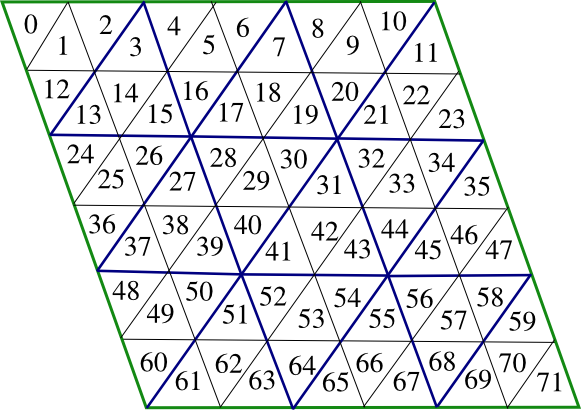
\includegraphics[width=7cm]{fig/IcosahedralGridCells.png}
	\caption{R3B2 decomposition of one of the parallelograms of the icosahedral. Blue lines show the first R3 decomposition, while black lines show the result of the additional B2 operation.}
	\label{fig:IcosahedralCells}
	\end{center}
\end{figure}

In this labelling, all the cells spin their upward, downward configuration in the grid, even when jumping to the next row. 
Least significant bit always identifies if the triangle is upward or downward.  
This layout of the blocks probably simplifies the looping along the cells when applying an operator. An example for the laplace follows
\begin{figure}[htb!]
\begin{minted}[
linenos,
numbersep=5pt,
frame=lines,
fontsize=\scriptsize,
framesep=2mm]{c++}
 // The following code shows only modifications to Mauro's triangular_storage
 // that works on the graph labelling studied here for two triangles of one of 
 // the icosahedral parallelograms
 struct triangular_offsets {
   int m_offset[3];
   static const int n_neighbors = 3;
   triangular_offsets(int a) {
     m_offset[0] = 1;
     m_offset[1] = -1;
     m_offset[2] = a;
   }
 
   int offset(int neighbor_index, int sign) const {
     return sign*m_offset[neighbor_index];
   }
 };
 
 template<typename OffsetFunction>
 struct triangular_storage {
 
 ...
   iterator begin() {
     return iterator(data.begin(), offset_function);
   }
   iterator operator++(int) const {
     return m_it+1;
   }
   iterator operator+(int i) const {
     return iterator(m_it+i, f, toggle_direction*(i&1 ? -1 : 1));
   }
   double& operator[](int i) {
     return *(m_it+f.offset(i, toggle_direction);
   }
   template <typename Functor>
   double fold_neighbors(iterator it, Functor && f) const {
     double v = 0;
     for (int i=0; i<OffsetFunction::n_neighbors; ++i) {
       v = f(v, it[i]);
     }
     return v;
   }
 };
 
 for (int i=1; i<n-1; ++i) {
 	for (int j=1; j<m-1; ++j) {
 		lap_cool.data[i*m+j] = 3*storage.data[i*m+j] -
 		storage.fold_neighbors(storage.begin()+i*m+j,
 		[](double state, double value) {
 			return state+value;
 		});
 	}
 }
\end{minted}
	\caption{Code example that illustrates the storace class and structure that defines the offset of neighbour cells, assuming an index layout like the one in figure~\ref{fig:IcosahedralCells} }
	\label{lst:TriangularOffsets}
\end{figure}

Figure also shows a possible way to tile the domain (in order to apply further parallelism) by always splitting into groups of two triangles with half size of the original parallelogram (figure~\ref{fig:IcosahedralTiling})

\begin{figure}[htb!]
	\begin{center}
		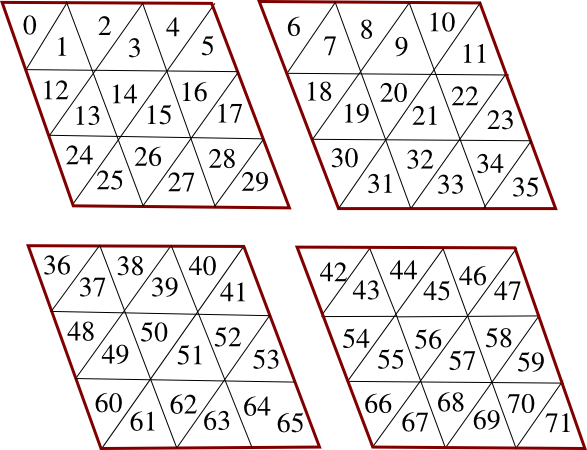
\includegraphics[width=7cm]{fig/IcosahedralGridTiling.png}
	\caption{One possible way of tiling an icosahedral parallelogram.}
	\label{fig:IcosahedralTiling}
	\end{center}
\end{figure}
\section{Vertexes and Edges Graph}

In addition to the graph of center of cells, ICON will probably need to consider the graph of vertexes (figure~\ref{fig:IcosahedralVertexes}) and edges (figure~\ref{fig:IcosahedralEdges}). Labeling of the nodes should allow to move
along these graphs in a consistent way. 
A stencil operating on fields in the mass point (cell graph) might require access
to the vertex graph storage or the edge graph storage. 
The data structure of the graph of cells could allow in the interface move into a 
different graph:

\begin{minted}[
linenos,
numbersep=5pt,
frame=lines,
fontsize=\scriptsize,
framesep=2mm]{c++}  
template<typename TEnv>
// structure that maps the cell graph into the vertex graph by
// providing the vertex ids around a cell id
//
// The VertexIdx is the index that identify one of the three vertexes that compose a triangle cell 
// The three vertexes of a cell are numbered like (for downward triangle)
//    (0)______(1)
//     \       /
//      \     /
//       \   /
//        \ /
//        (2)
//    
// or for upward triangle
//
//         (0)
//         / \
//        /   \
//       /     \
//      /_______\
//    (2)       (1)
//
//    
struct cell_map {
  int m_offsets[6];
  static const int n_vertexes = 3;
  cell_map(int a) {
      m_offset[0] = 0;
      m_offset[1] = 1;
      m_offset[2] = a/2;
      m_offset[3] = 0;
      m_offset[4] = a/2+1;
      m_offset[5] = a/2;
  }
  // the following computes the vertex index of one of the vertexes
  // (determined by VertexIdx) of a cell (CellIdx)
  // Same idea should work with iterators 
  int vertex_index(const int VertexIdx, const int CellIdx){
    return (CellIdx+1)/2+CellIdx/a + m_offset[VertexIdx+n_vertexes*(CellIdx&1)];
  } 
};

// structure that maps the cell graph into the edges graph by
// providing the edges ids around a cell id
//
// The EdgeIdx is the index that identify one of the three edges that compose a triangle cell 
// The three edges of a cell are numbered like, for downward triangle
//     ____(1)___
//     \        /
//      \      /
//      (0)  (2)
//        \  /
//         \/
//        
//    
// or for upward triangle
/*
//          /\
//         /  \
//       (0)  (1)
//       /      \
//      /___(2)__\
*/           

struct cell_map {
  int m_offsets[6];
  static const int n_edges = 3;
  cell_map(int a) {
      m_offset[0] = 0;
      m_offset[1] = 1;
      m_offset[2] = 2;
      m_offset[3] = -1;
      m_offset[4] = 0;
      m_offset[5] = a/2*3-1;
  // the following computes the edge index of one of the edges 
  // (determined by EdgeIdx) of a cell (CellIdx)
  int edge_index(const int EdgeIdx, const int CellIdx){
      return ((CellIdx+1)/2*3) + CellIdx/a + m_offset[EdgeIdx+n_edges*(CellIdx&1)];
  }
};
\end{minted}



\begin{figure}[htb!]
	\begin{center}
		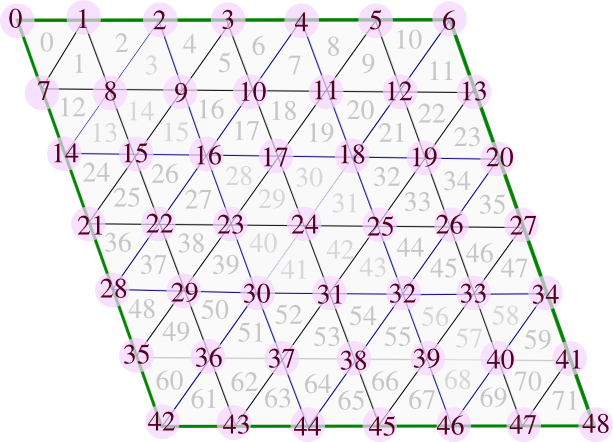
\includegraphics[width=7cm]{fig/IcosahedralGridVertexes.png}
	\caption{Graph of icosahedral vertexes.}
	\label{fig:IcosahedralVertexes}
	\end{center}
\end{figure}

\begin{figure}[htb!]
	\begin{center}
		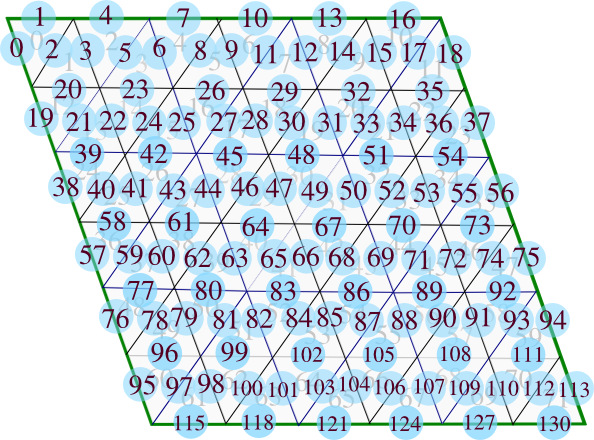
\includegraphics[width=7cm]{fig/IcosahedralGridEdges.png}
	\caption{Graph of icosahedral edges. Note that the nodes in the last row
		show discontinuous index labelling in order to keep a consistent mapping between the graph of cells and the graph of edges. This requires adding some padding to the data structures.}
	\label{fig:IcosahedralEdges}
	\end{center}
\end{figure}

Also we, similarly to triangular\_offsets, each node of the vertex and edge graph should be able to (random) access and iterate over its neighbours. 
The following structure show how we can access the neighbours for the layout 
drawn in figure~\ref{fig:IcosahedralVertexes} and~\ref{fig:IcosahedralEdges}:

\begin{minted}[
linenos,
numbersep=5pt,
frame=lines,
fontsize=\scriptsize,
framesep=2mm]{c++}
//
//  indexes to refer to a vertex
//      0_______1
//     /         \
//    /           \
//   /             \
//  5      ref      2
//   \             /
//    \           /
//     \         /
//      4_______3 

struct vertex_neighbour_offsets {
  int m_offsets[6];
  static const int n_neighbours = 6;
  vertex_neighbour_offsets(int a) {
    m_offset[0] = -a/2-1;
    m_offset[1] = -a/2;
    m_offset[2] = 1;
    m_offset[3] = a/2+1;
    m_offset[4] = a/2;
    m_offset[5] = -1;
  }
  // vertexes at the corners of the parallelogram will have only 5 neigoubrs
  // i.e. vertexes 0, 6, 42, 48 
  // we will have to deal with these exceptional cases once we build halos around
  // the parallelogram
  int vertex_offset(int neighbour_index){
    return m_offset[neighbour_index];
  }
};
\end{minted}

\begin{minted}[
linenos,
numbersep=5pt,
frame=lines,
fontsize=\scriptsize,
framesep=2mm]{c++}
// There are three different shapes of parallelograms of edges with different
// neighbours relations. The neigbour index will is depicted below for each
// type of edge parallelogram
// 
//      type I
//
//      _____1____
//     /\        /
//    /  \      /
//   0   ref   2
//  /      \  /
// /____3___\/ 
//
// 
//     type II
//
//  _____1____
//  \        /\
//   \      /  \
//    0   ref   2 
//     \  /      \
//      \/____3___\
//
//
//      type III
//
//        /\
//       /  \
//      0    1
//     /      \
//    /__ref __\
//    \        /
//     \      /
//      3    2
//       \  /
//        \/
//
struct edge_neighbour_offsets {
  int m_offsets[4];
  static const int n_neighbours = 4;
  edge_neighbour_offsets(int a) {
    m_offset[0] = -1;
    m_offset[1] = 1;
    m_offset[2] = 2;
    m_offset[3] = a/2*3-1;
    m_offset[4] = -2;
    m_offset[5] = -1;
    m_offset[6] = 1;
    m_offset[7] = a/2*3;
    m_offset[8] = -a/2*3;
    m_offset[9] = -a/2*3;
    m_offset[10] = 1;
    m_offset[11] = -1;
  }
  int edge_offset(const int neighbour_index, const int type){
    return m_offset[neighbour_index+type*n_neighbours];
  }
};
\end{minted}

\section{Domain Decomposition and Halos}

The original indexing proposed in figure~\ref{fig:IcosahedralCells} does not take into account halo regions, which will be essential in a block structured code.
Adding halo regions around each parallelogram domain requires a well defined distribution of
these parallelogram domains that fill the whole sphere. 
%In figure~\ref{fig:IcosahedralDecomposition} we take the global domain %decomposition and diamonds labeling from GME.

Figure~\ref{fig:IcosahedralDiamondWithHalos} shows an schema for numbering
cells 
in a consistent way (similar to figure~\ref{fig:IcosahedralCells}) but considering
halo cells.
Grid vertices at the corners of the diamond always have 5 surrounding cells, while
all the other vertices in the grid contain 6 cells around.

\begin{figure}[htb!]
	\begin{center}
		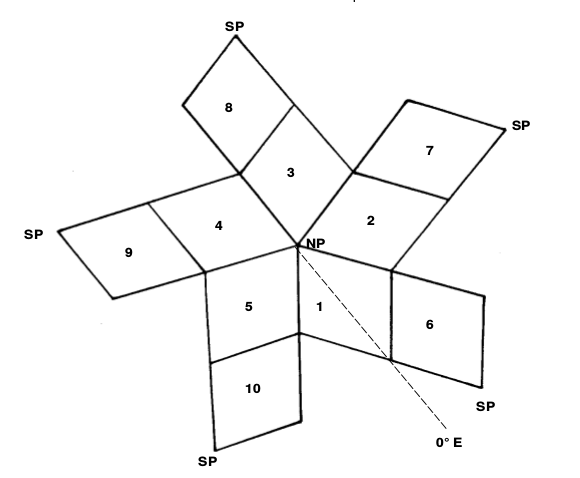
\includegraphics[width=14cm]{fig/IcosahedralDecomposition.png}
		\caption{Domain decomposition of a icosahedron grid into ten diamonds.
			Five of these contain the north pole, the other five the south pole}
		\label{fig:IcosahedralDecomposition}
	\end{center}
\end{figure}

\begin{figure}[htb!]
	\begin{center}
		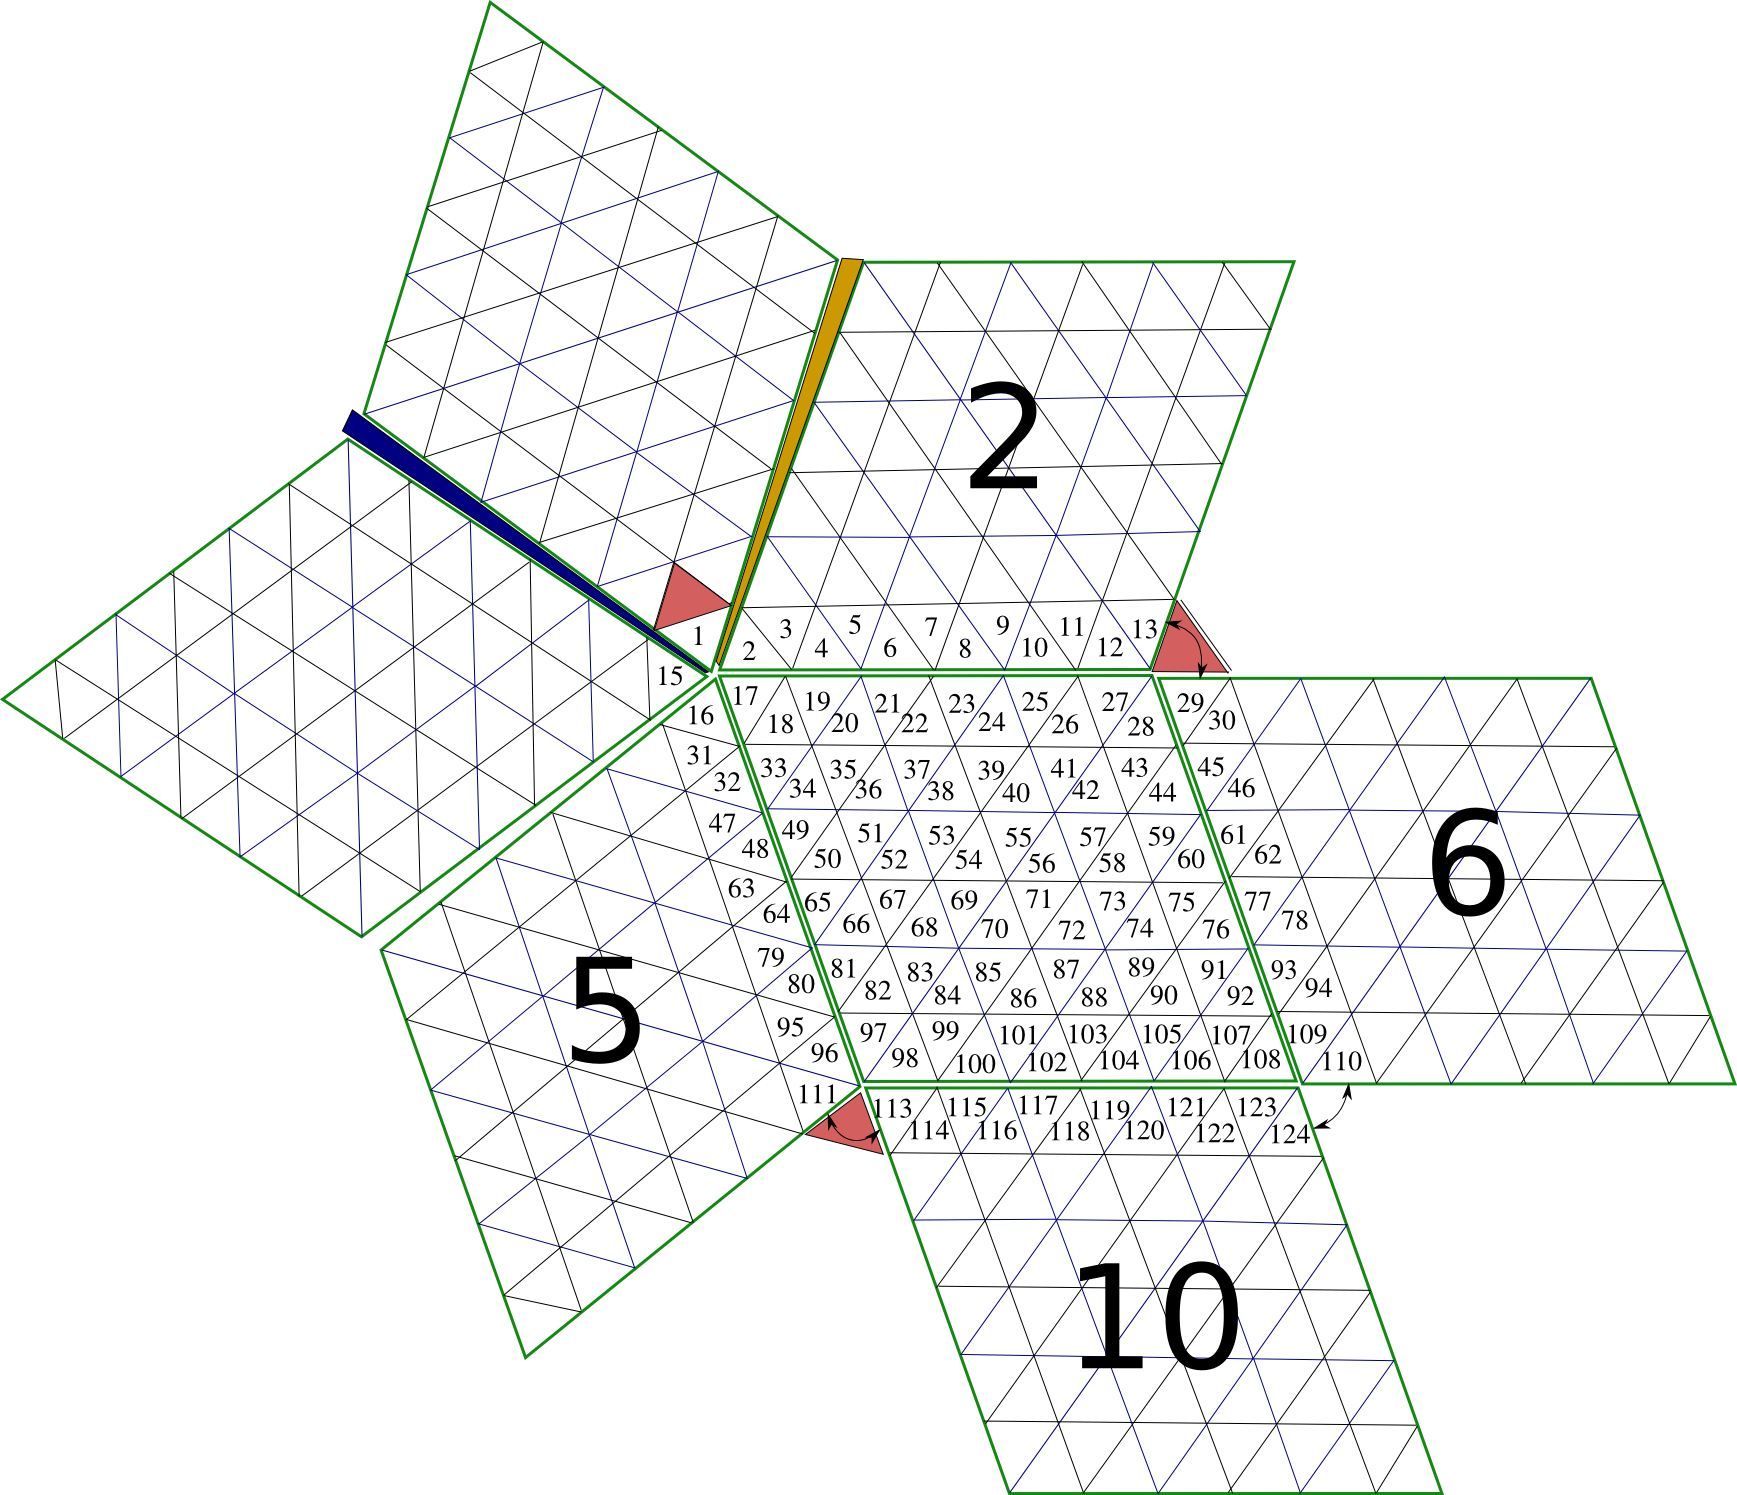
\includegraphics[width=18cm]{fig/IcosahedralGridCellHalos_v2.png}
		\caption{
			Grid cells labeling of one of the original diamonds containing
	halo regions with 2 neighbour cells at the halos. 
	Red triangle represents padding cells required to keep consistency of strides
	along the different rows of the diamond. Each diamond of the original icosahedron 
	decomposition is identified with the label convention followed in figure~\ref{fig:IcosahedralDecomposition}.
	Arrows indicate neighbour relation between two cells which are not contiguous in the indexing space (there is some padding).
	The blue wedge indicates a transition between two regions that do
	not respect the neighborhood rules of cells.
	Yellow wedge indicates a transition between triangles where 
	contiguous downward/upward swap is not respected (i.e. triangles 1 and 2 are both upward). Special care must be taken when jumping into a padding cell, following any of the arrows connecting two cells and/or crossing any of the two wedges. In that case the neighborhood rules dictated by triangular\_offsets in~\autoref{lst:TriangularOffsets} are not respected. 
 	}
	\label{fig:IcosahedralDiamondWithHalos_1}
	\end{center}
\end{figure}

\begin{figure}[htb!]
	\begin{center}
		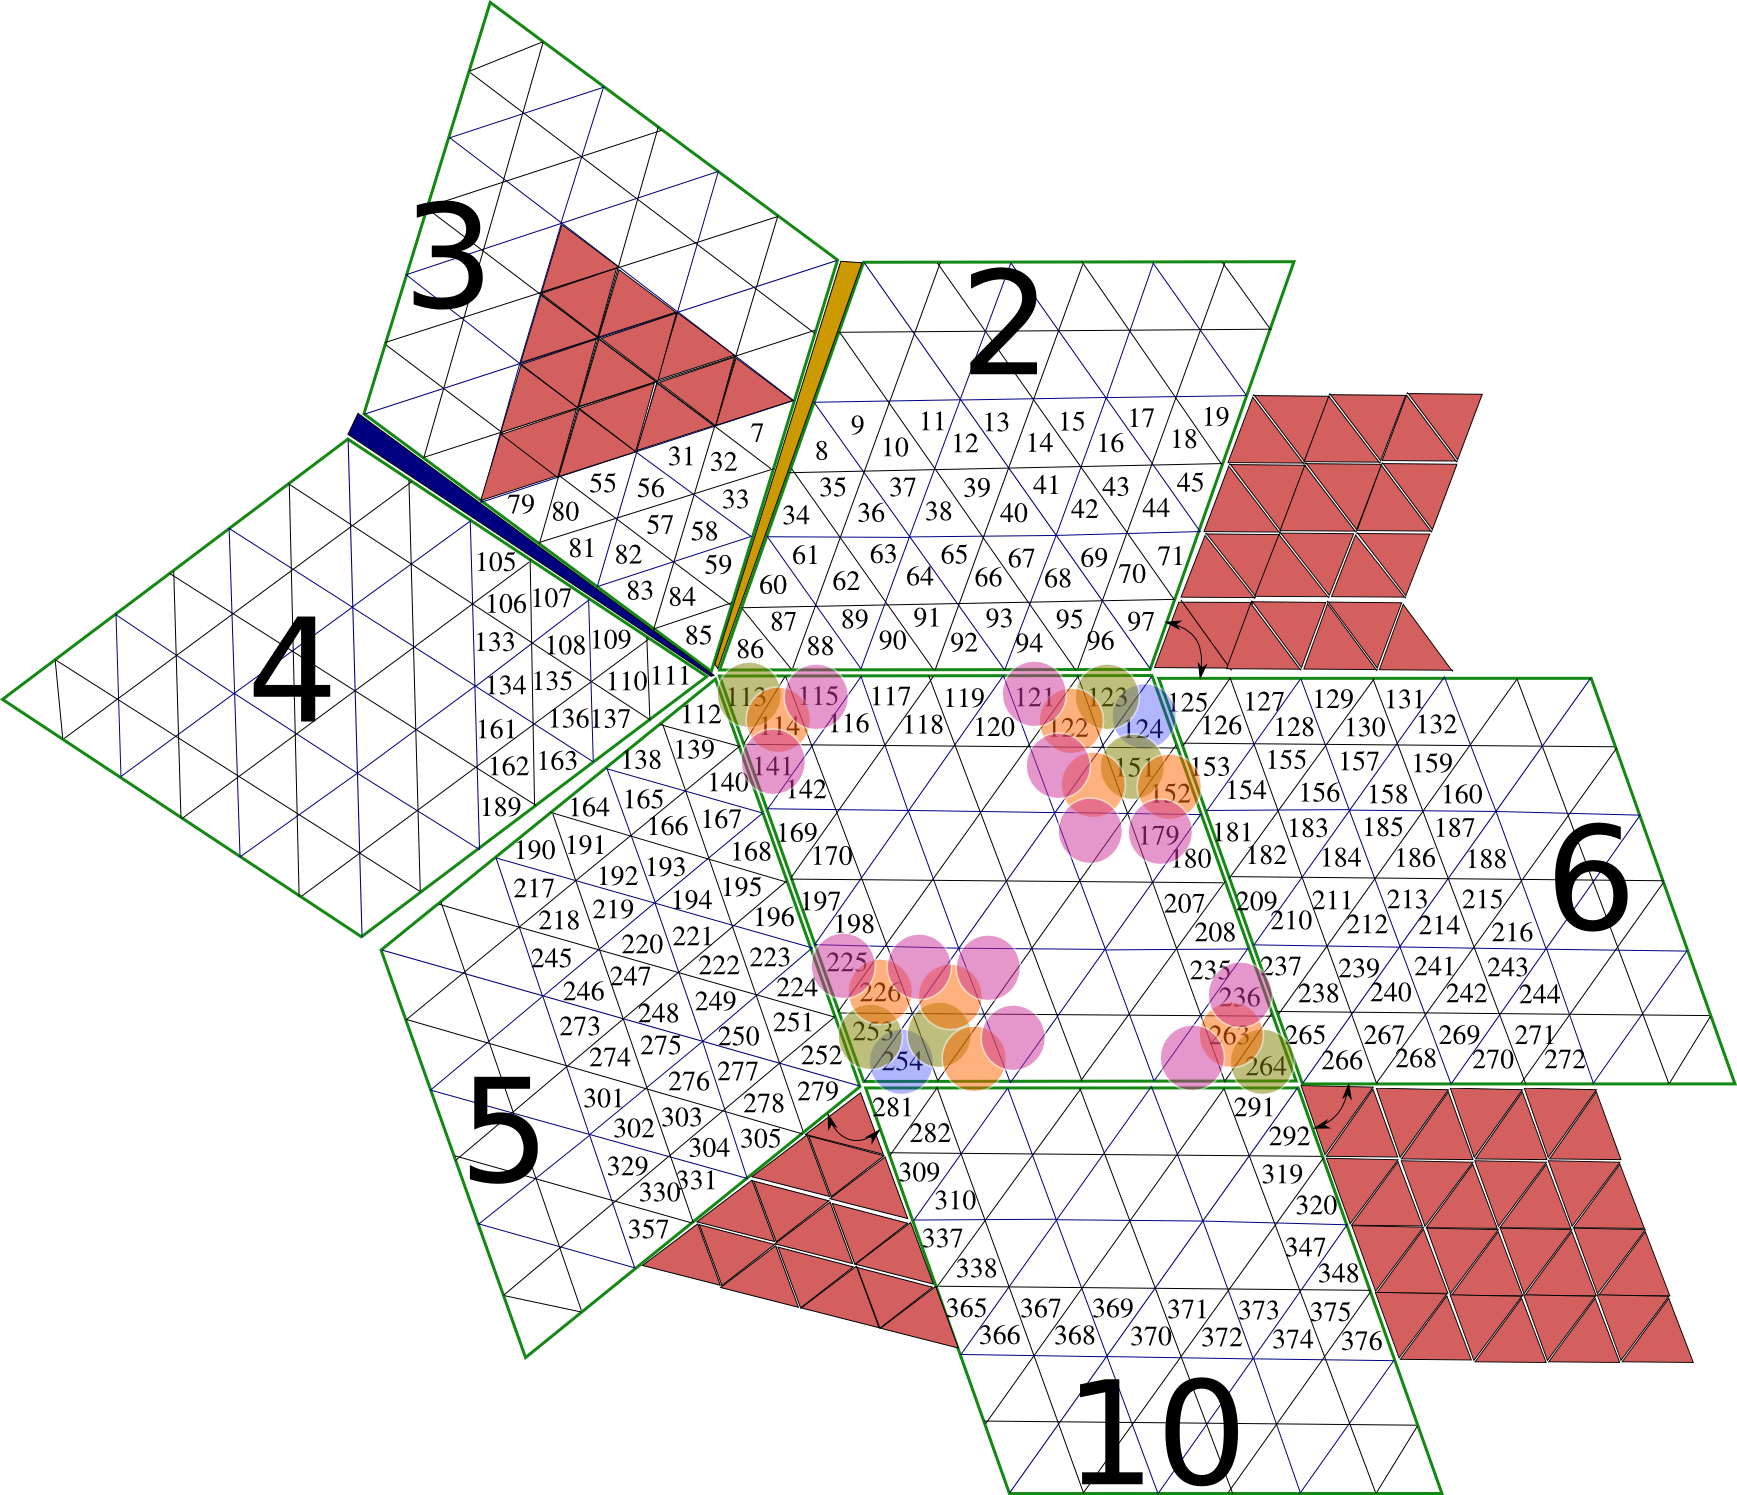
\includegraphics[width=18cm]{fig/IcosahedralGridCellHalos8_v2.png}
		\caption{
		Same as~\autoref{fig:IcosahedralDiamondWithHalos_1} with 4 halo lines. 
		Red triangle represents padding cells required to keep consistency of strides
		along the different rows of the diamond. Each diamond of the original icosahedron 
		decomposition is identified with the label convention followed in figure~\ref{fig:IcosahedralDecomposition}.
		Arrows indicate neighbour relation between two cells which are not contiguous in the indexing space (there is some padding).
		The blue wedge indicates a transition between two regions that do
		not respect the neighborhood rules of cells.
		Yellow wedge indicates a transition between triangles where 
		contiguous downward/upward swap is not respected (i.e. triangles 1 and 2 are both upward). Special care must be taken when jumping into a padding cell, following any of the arrows connecting two cells and/or crossing any of the two wedges. In that case the neighborhood rules dictated by triangular\_offsets in~\autoref{lst:TriangularOffsets} are not respected.
		None of the cells in the computation domain can cross any of
		these regions (or fall into a padding cell) with one neighbour move. 
		Blue circles mark cells which can cross one of these regions (or fall into a padding cell) in which case the general offset rule is not respected with two neighbour moves.
		Green circles need three neighbour moves. Orange circles need 4 neighbour moves and finally magenta need 5. 
		}
		\label{fig:IcosahedralDiamondWithHalos_4}
	\end{center}
\end{figure}


Indexing schema shown in figure~\ref{fig:IcosahedralDiamondWithHalos} shows that all of the cells need the same offsets in order to access any of the three neighbouring cells (padding is required in order to achieve that). This is also true for most of the cells in the halos. 
However there are three cells around the corners of the diamond, enclosed in blue circles in figure~\ref{fig:IcosahedralDiamondWithHalos}, 
which require different offsets. I.e. the triangular\_offsets defined in figure~\ref{lst:TriangularOffsets} is not valid for those cells under blue circles. These grid cells will require special treatment.
 
This can also impose some restrictions, also on cells inside the computation domain in case operators of order greater than one are used\footnote{This refer to high order operators which are computed on the fly. 
For example a fourth order horizontal diffusion can be computed as 
two laplace operators concatenated via a temporary field, or as two nested
laplace stencil functions. The first case should never be a limitation here, as
each operator will only access first order neighbours.}
For example if second order operators are defined by the user, i.e. stencils
that access second order neighbours, the corner cells 17, 28 and 98 will 
also require special treatment. 

\begin{figure}[htb!]
	\begin{center}
		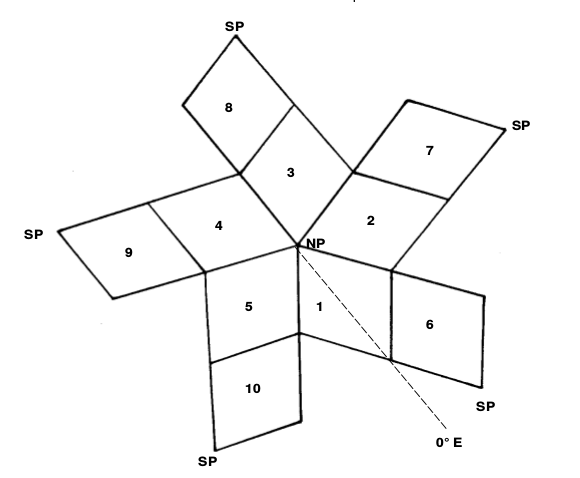
\includegraphics[width=14cm]{fig/IcosahedralDecomposition.png}
		\caption{Domain decomposition of a icosahedron grid into ten diamonds.
			Five of these contain the north pole, the other five the south pole}
		\label{fig:IcosahedralDecomposition}
	\end{center}
\end{figure}

\begin{figure}[htb!]
	\begin{center}
		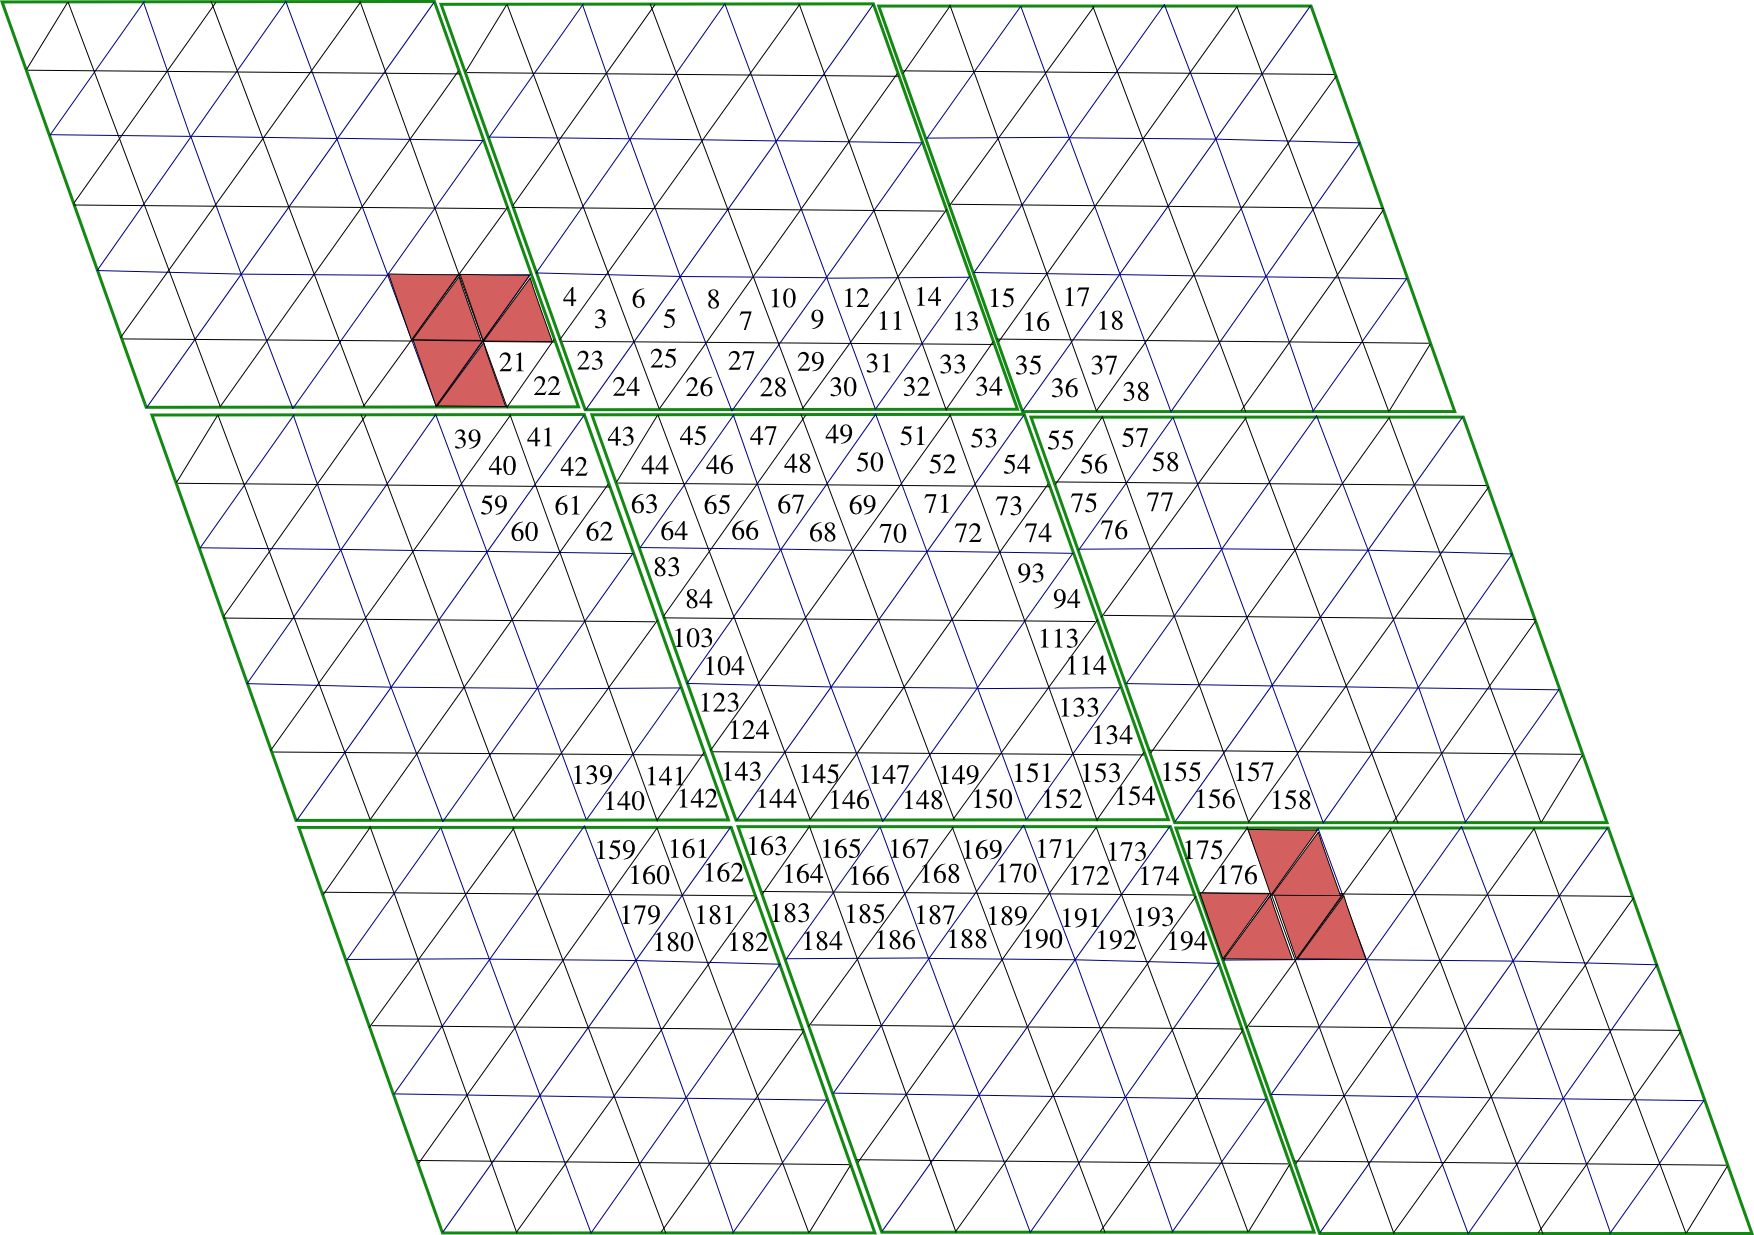
\includegraphics[width=18cm]{fig/IcosahedralGridCellHalosInnerDiamond.png}
		\caption{Grids cells labeling of an inner diamond, where none 
			of the corners is a corner of an diamond of the original 
			decomposition of the icosahedron (figure~\ref{fig:IcosahedralDecomposition}).
			Red cells indicate required padding in order to keep uniform offset rules accross the domain. 
			In this case, all the cells exhibit exactly the same neighbour cells relationship (i.e. describe with a unique offset for the whole domain and halos). No exceptional treatment of some cells is required.
		}
		\label{fig:IcosahedralDiamondWithHalosInnerDiamond}
	\end{center}
\end{figure}

In case one of the original diamonds in figure~\ref{fig:IcosahedralDecomposition} is further decomposed, the corner vertices
of the resulting diamond is always composed by six neighbour cells
(see figure~\ref{fig:IcosahedralDiamondWithHalosInnerDiamond}).
In this case, the offset pattern of neighbour is always applicable for all the grid cells (included halo cells).


\bibliographystyle{abbrv}

\bibliography{references}{}

\end{document}


